\documentclass{article}

\usepackage{fancyhdr}
\usepackage{extramarks}
\usepackage{amsmath}
\usepackage{amsthm}
\usepackage{amsfonts}
\usepackage{tikz}
\usepackage[plain]{algorithm}
\usepackage{algpseudocode}

\usetikzlibrary{automata,positioning}

%
% Basic Document Settings
%

\topmargin=-0.45in
\evensidemargin=0in
\oddsidemargin=0in
\textwidth=6.5in
\textheight=9.0in
\headsep=0.25in

\linespread{1.1}

\pagestyle{fancy}
\lhead{The University of Adelaide}
\rhead{COMP SCI 3315 - Computer Vision}
\lfoot{Nathaniel Chang (a1821595)}
\cfoot{}
\rfoot{\thepage}

\renewcommand\headrulewidth{0.5pt}
\renewcommand\footrulewidth{0.5pt}

\setlength\parindent{0pt}
\setlength{\parskip}{\baselineskip}% 

%
% Homework Details
%   - Title
%   - Date
%   - Class
%   - Author
%

\newcommand{\hmwkName}{\textbf{\huge Assignment 3 - Question 2}}
\newcommand{\hmwkDueDate}{May 20, 2024}
\newcommand{\hmwkClass}{COMP SCI 3315 - Computer Vision}
\newcommand{\hmwkAuthorName}{\textbf{Nathaniel Chang (a1821595)}}

%
% Title Page


\renewcommand{\maketitle}{

	\hmwkName \\
	\vspace{0.01cm} \\
	\hmwkClass \\
	\hmwkDueDate \\
	\hmwkAuthorName \\
	
	\vspace{1cm}
    
}

\begin{document}

\maketitle

\section{Introduction}

It can be hard and expensing to capture high resolution images but the higher the resolution of an image the better clarity and detail we are able to see in the image. Having high resolution images in many different fields is import including medical imaging, satellite imaging, and film restoration. These images are able to provide a better user experience and analytic insights, hence the need for high resolution images.

\section{Defining the Computer Vision Problem / Area}

To increase the resolution of an image an increase to the number of pixels is required to enhance the detail and the clarity of an image. There are two methods traditional interpolation and deep networks. Interpolation involves estimating the pixels between the existing pixels which can lead to the problems like loss of detail, aliasing, and limits on the scalability. While deep network are trying to predict the missing pixels with a CNN (Convolutional Neural Network), which leads to better scalability, and high quality results \cite{medium1}. Increasing the images resolution is also able to help other Computer vision including image recognition and object detection. This also benefits the medial imaging field where the clarity in images is crucial in being able to detect different problem and diseases.


\section{Application Scenarios}

In medical imaging a lot of detail is needed in these images so that medical professionals are able to make accurate diagnosis based on the information in front of them. The more information that they are able to get out of an image the more accurate they can be. The cost of such large images can be high so using upscaling medical professionals would be able to get better images for less cost \cite{Ahmad2022}.

Satellite Imaging is another great application for image upscaling, even though cameras in satellites are able to capture high resolution images. Sometimes the user needs more pixels to be able to complete the task that they are working on. Using Image Upscaling more pixels would could be predicted and users would be able to use them to complete those tasks demanding higher resolution images \cite{Buczkowski2023}.

Film restoration is another application for image upscaling, to use the techniques to predict pixels that might be missing. Restoring and improving these old films allow users to keep these parts of history alive for generations to come \cite{MACHIDON2018181}.

\section{Solution Overview}

There are a couple of different solutions that are going to be covered, traditional methods (bilinear and bicubic interpolation) and advance techniques (Convolution Neural Networks).

Traditional Methods, both bilinear and bicubic are similar but there are differences. Bilinear is assuming that there is a linear change from pixel to pixel. Bicubic takes the intensity of the neighbouring pixels to create a smooth curve seen in figure \ref{fig:bilin_bicub}.

\begin{figure}[h]
    \centering
    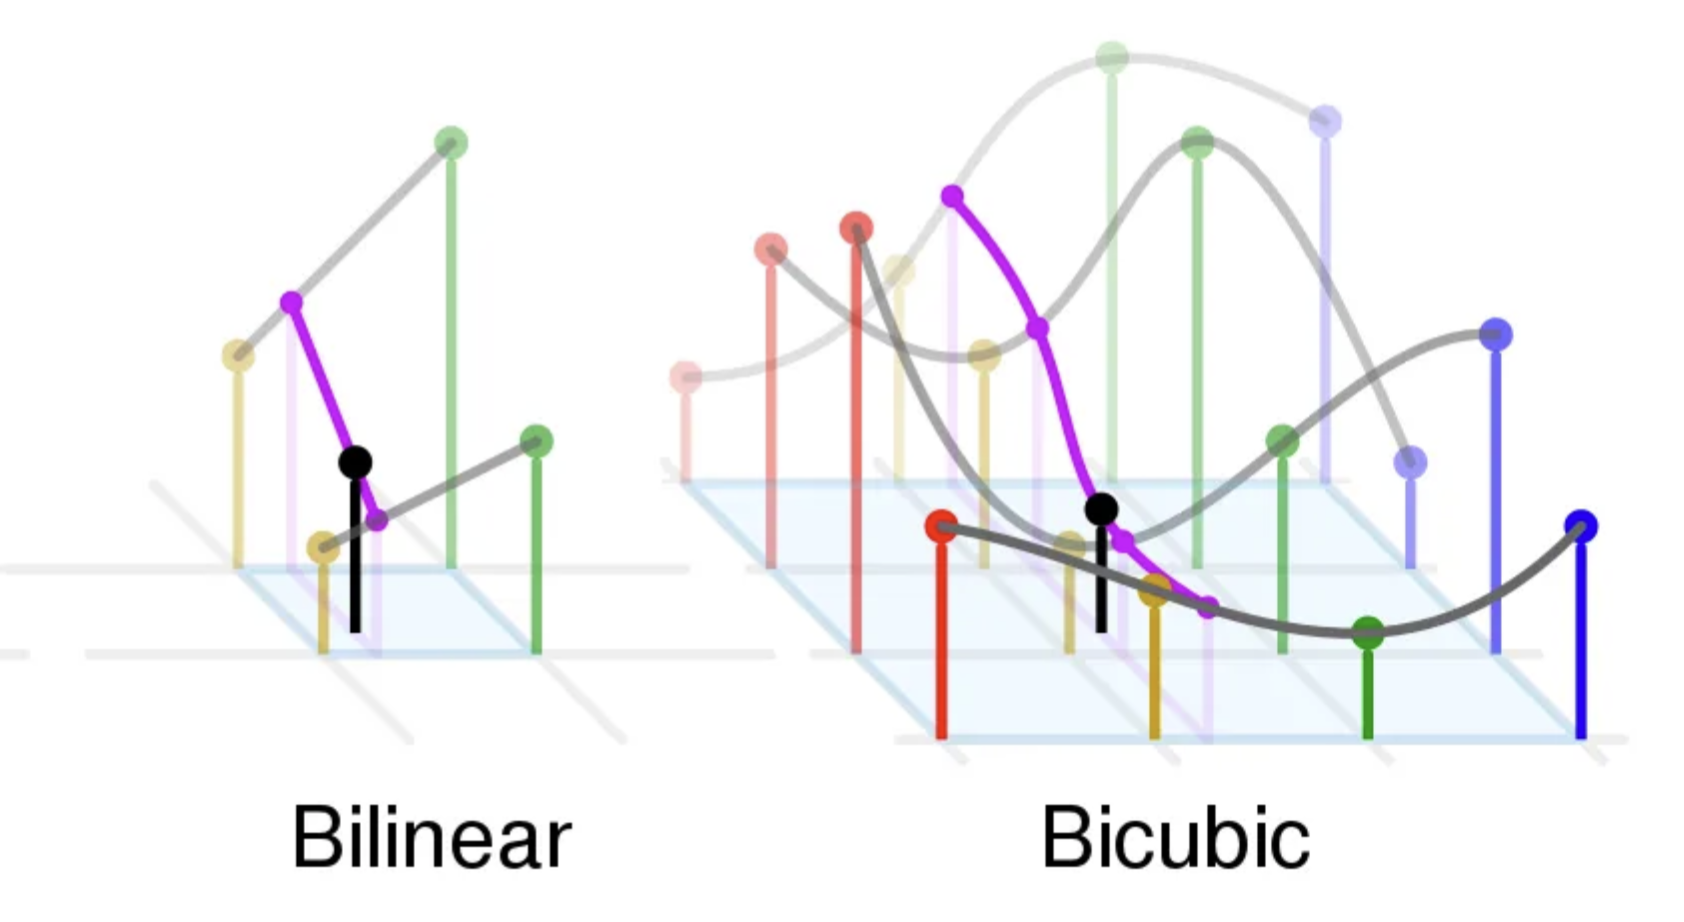
\includegraphics[width=0.5\textwidth]{bilinear_bicubic}
    \caption{3d Digram of Bilinear and Bicubic \cite{rao2023image}}
    \label{fig:bilin_bicub}
\end{figure}

Using advance techniques, convolution neural networks are a deep learning technique that are able to be used for image upscaling. The goal of the CNN is to reduce the input to a smaller matrix, while trying to keep the features. With this they are able to detect patterns and features in the image. Through out the reduction of the layers filters are applied to the input, that will capture features such as textures, edges, and spaces please see figure \ref{fig:cnn} for an example structure of a CNN.

\begin{figure}[h]
    \centering
    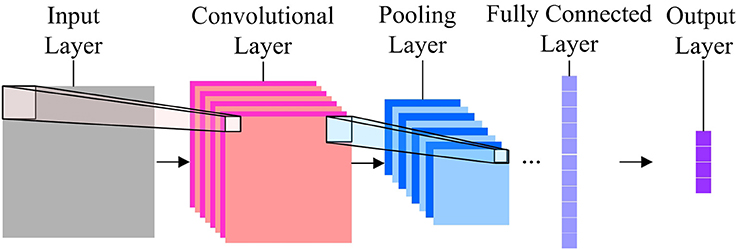
\includegraphics[width=0.5\textwidth]{fpsyg-08-01745-g001}
    \caption{Example structure of a CNN \cite{10.3389/fpsyg.2017.01745}}
    \label{fig:cnn}
\end{figure}

\section{Advantages and Limitations}

There are many advantages of using CV techniques for image upscaling, these include improved details and clarity within image, if using bilinear and bicubic interpolation they are be easy to implement. CNN can also be fast after they have been trained, there other advantage is that they are able to be trained on specific tasks eg medical imaging or satellite images.

There are also limitations to using these techniques in these applications. There risk or artefacts and unrealistic detail as pixels are getting predicted and weren't captured with the sensor these models could create details that don't actually exist see figure \ref{fig:atrifacts} and \ref{fig:brain}. In medical imaging we wouldn't want to create details in the image that doesn't exist. High computational requirements and the performance depends on training data are other limitations. Training these model sometimes need high performance computers so that computational time isn't that long. As these models are predicting pixels if the training data isn't great then the model won't be able to predict the pixels as well.

\begin{figure}[h]
    \centering
    
\includegraphics[width=0.5\textwidth]{changi-screenshot-xb87u3E1@2x}
    \caption{Example of artifacts with bilinear and bicubic interpolation \cite{Jensen2017}}
    \label{fig:atrifacts}
\end{figure}

\begin{figure}[h]
    \centering
    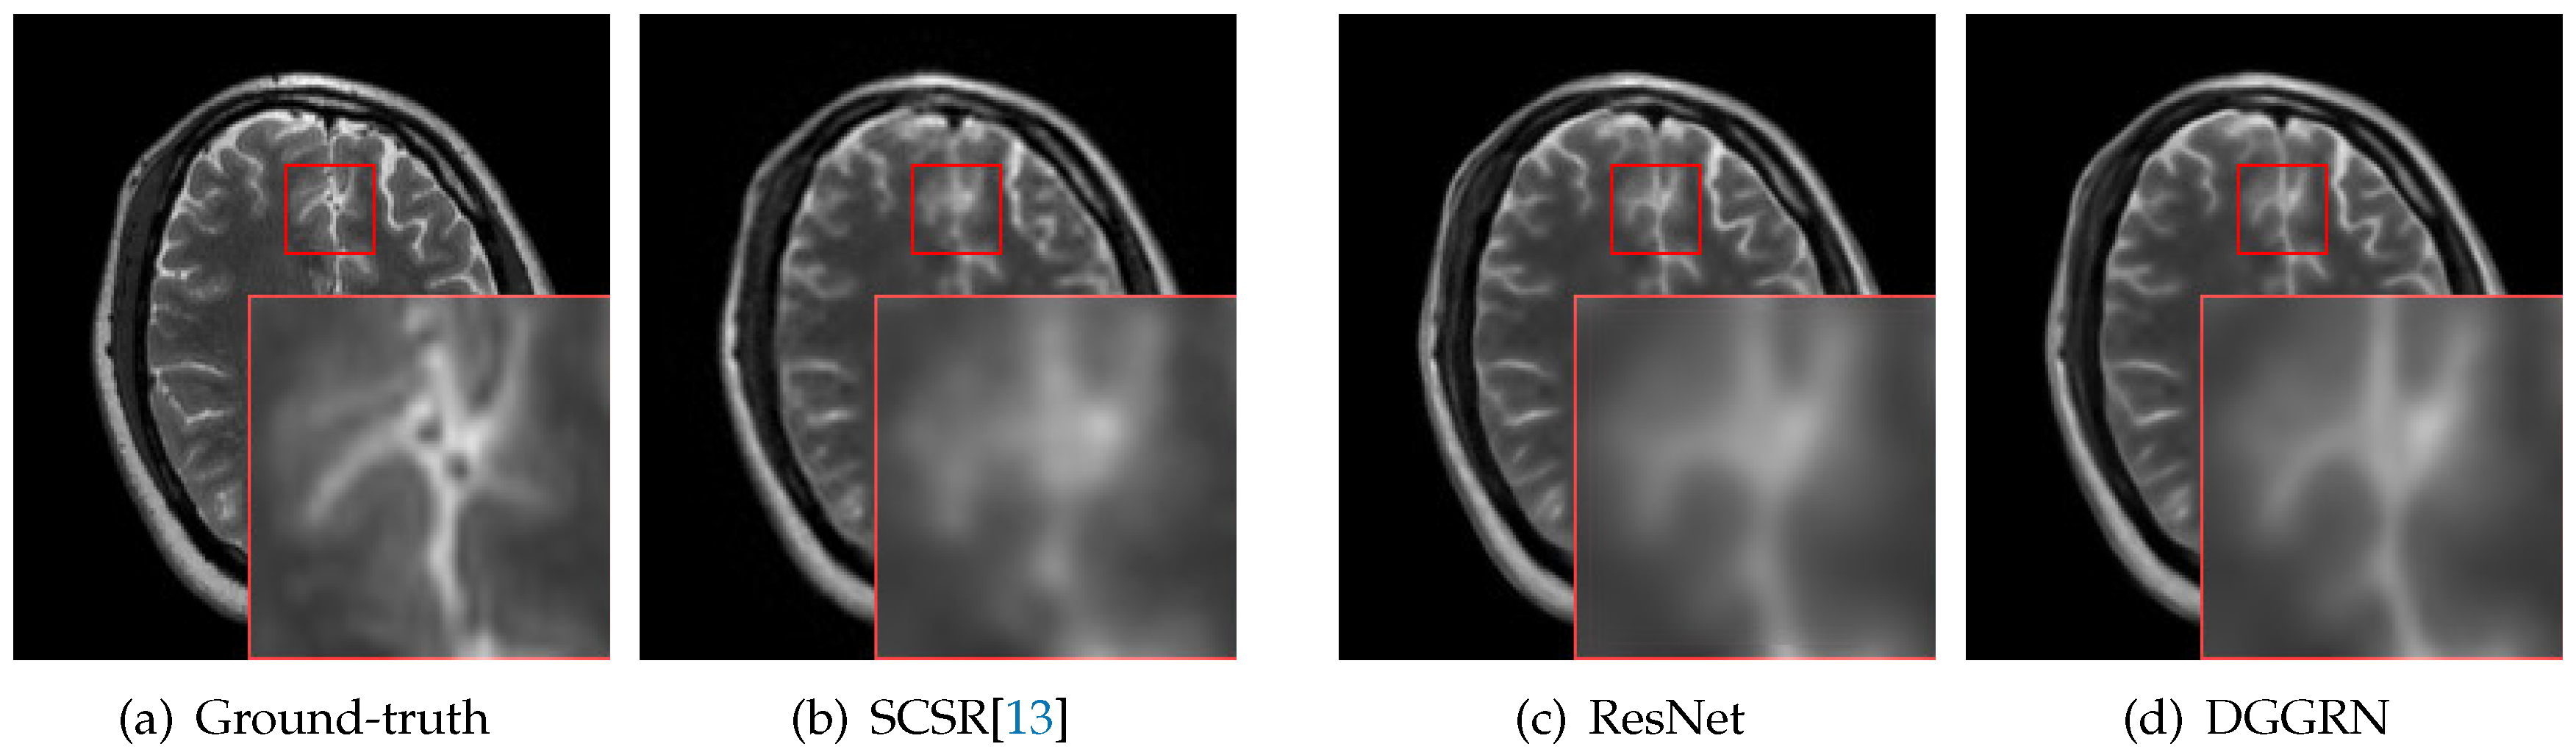
\includegraphics[width=0.7\textwidth]{applsci-09-04874-g001}
    \caption{Example of errors when upscalling with a CNN \cite{Du2019}}
    \label{fig:brain}
\end{figure}


\section{Conclusion}

There are many applications for image upscaling medical imaging, satellite imagery, and film restoration to name a few. There are defiantly advantages and disadvantages of them but they are promising aspects and over time they will only get better for these applications. 


\bibliography{references.bib}
\bibliographystyle{IEEEtran}


\end{document}
